% !Mode:: "TeX:UTF-8"
\chapter{SQLite数据库的web移植}

\section{SQLite简介}

SQLite是一款轻量、高速的可嵌入式数据库\upcite{junyan2009application}。
作为一个完整的关系型数据库管理系统,虽然SQLite很轻量小巧,还是遵守ACID规范。
SQLite和Lua虚拟机一样,完全由POSIX C写成,同样没有其他第三方依赖
它是D.RichardHipp建立的公有领域项目。
SQLite最初的目标平台是嵌入式卡片机,而且很多嵌入式设备(比如索尼的PSP/PSV,任天堂的NDS/3DS)和软件 (如android和unity3D) 都内置了SQLite用来管理各种信息。它的硬件需求非常的低,只需要数百KB的内存就足够运行,非常适合在嵌入式系统和低配置设备中使用。

SQLite能够支持所有POSIX兼容系统,比如常见的Windows/Linux/BSD等主流操作系统,并且编程接口齐全,能很好的与众多的编程语言相结合,比如Java、Python、Ruby、PHP等语言,而且大部分语言都有ODBC接口。在关系型数据库中,SQLite和另外两个业界重量级开源关系型数据库相比较,它的处理速度比他们都快。不过SQLite只实现了ANSI SQL,并没有其他的SQL扩展。至2016年已经有16个年头,SQLite重大更新的SQLite 3则更新于2015年。现在,SQlite已经成为了分发数量最多的数据库引擎。

一般的数据库引擎都使用Client/Server架构,但是SQLite不是。RichardHipp在SQLite引擎时不希望其作为一个服务,而且像Lua虚拟机那样,可以嵌入到应用程序之中进行运行。在SQLite嵌入到应用程序的情况下,所有的信息交换都在应用程序内部进行,编程语言可以直接使用API接口对SQLite的数据进行操作,而不需要外部通讯。极大降低了硬件的需求,显著减少了通讯延迟,还能简化数据库系统本身的设计。整个数据库使用单一文件的形式进行保存,整个数据库的表、索引和数据都保存在一个静态文件中,也可以很方便的进行数据库的共享和迁移。而且,事物范围也可以有明确的约束。

SQLite单文件的特性,使html5 filesystem API\upcite{bidelman2011using}
模拟实现有了理论上的可能。

\section{SQLite的程序的特征}

和lua虚拟机相同,SQLite我们也是需要得到一个“黑箱程序”即可。
但SQLite又和luaVM有个显著的不同,数据库一般都是C/S架构的,但SQLite不是,
所以我们不需要在前端模拟实现C/S架构。

Html5中新增了原生的前端多线程方案,Web Worker\upcite{jarvinen2011html5},
依靠线程间通信,可以显著提高查询时运行的效率。因为SQLite是阻塞的,而JavaScript是异步语言。

\section{SQLite程序的移植过程}

\subsection{SQLite程序的移植过程}

SQLite程序的移植过程如下所示:

\begin{enumerate}[itemindent=2em]
    \item 下载SQLite生成用c源码,只有一个c文件和一个头文件;
    \item 把sqlite3.c和sqlite3.h两个文件放在c文件夹下,然后编写如下makefile;
\begin{verbatim}
# Need $(EMSCRIPTEN), for example run with        emmake make

EMSCRIPTEN?=/usr/bin

EMCC=$(EMSCRIPTEN)/emcc

CFLAGS=-DSQLITE_OMIT_LOAD_EXTENSION -DSQLITE_DISABLE_LFS -
	DLONGDOUBLE_TYPE=double -DSQLITE_INT64_TYPE=
	"long long int" -DSQLITE_THREADSAFE=0

all: js/sql.js

debug: EMFLAGS= -O1 -g -s INLINING_LIMIT=10 
debug: js/sql-debug.js

optimized: EMFLAGS= --memory-init-file 0 --closure 1 -O3 -s INLINING_LIMIT=50
optimized: js/sql-optimized.js

js/sql.js: optimized
	cp js/sql-optimized.js js/sql.js

js/sql%.js: js/shell-pre.js js/sql%-raw.js js/shell-post.js
	cat $^ > $@

js/sql%-raw.js: c/sqlite3.bc js/api.js exported_functions
	$(EMCC) $(EMFLAGS) -s EXPORTED_FUNCTIONS=
		@exported_functions c/sqlite3.bc --post-js js/api.js -o $@

js/api.js: coffee/api.coffee coffee/exports.coffee coffee/api-data.coffee
	coffee --bare --compile --join $@ --compile $^

# Web worker API
worker: js/worker.sql.js
js/worker.js: coffee/worker.coffee
	coffee --bare --compile --join $@ --compile $^

js/worker.sql.js: js/sql.js js/worker.js
	cat $^ > $@

c/sqlite3.bc: c/sqlite3.c
	# Generate llvm bitcode
	$(EMCC) $(CFLAGS) c/sqlite3.c -o c/sqlite3.bc

module.tar.gz: test package.json AUTHORS README.md js/sql.js
	tar --create --gzip $^ > $@

clean:
	rm -rf js/sql*.js js/api.js js/sql*-raw.js c/sqlite3.bc
\end{verbatim}    	
	\item 运行make命令,得到sql.js文件;
	\item 使用sql.js。
\end{enumerate}



\subsection{SQLite程序的移植过程分析}

SQLite的程序的移植过程分析,即该makefile作用如下:

\begin{enumerate}[itemindent=2em]
    \item 把sqlite.c文件编译成sqlite.bc文件,即为llvm的字节码;
    \item api.coffee,exports.coffee,api-data.coffee文件编译成api.js,coffeescript是一种脚本语言,可以编译成JavaScript,写作方式类似python;
    \item sqlite.bc编译成sql-optimized-raw.js,需要api.js辅助;
	\item 把shell-pre.js,sql-optimized-raw.js,shell-post.js合并,其中shell-pre和shell-post两个js文件是用来修饰SQLite的使用方法,使之在html和node.js中调用更方便;
	\item 优化sql-optimized-raw.js,得到sql-optimized.js;
	\item 将sql-optimized.js改名为sql.js。
\end{enumerate}

\subsection{SQLite在浏览器中的运行效果}

图\ref{sqlite-html}展示了SQLite在浏览器中运行的效果。

\begin{figure}[h!] % [h!] 表示尽量排在当前位置
    \centering
    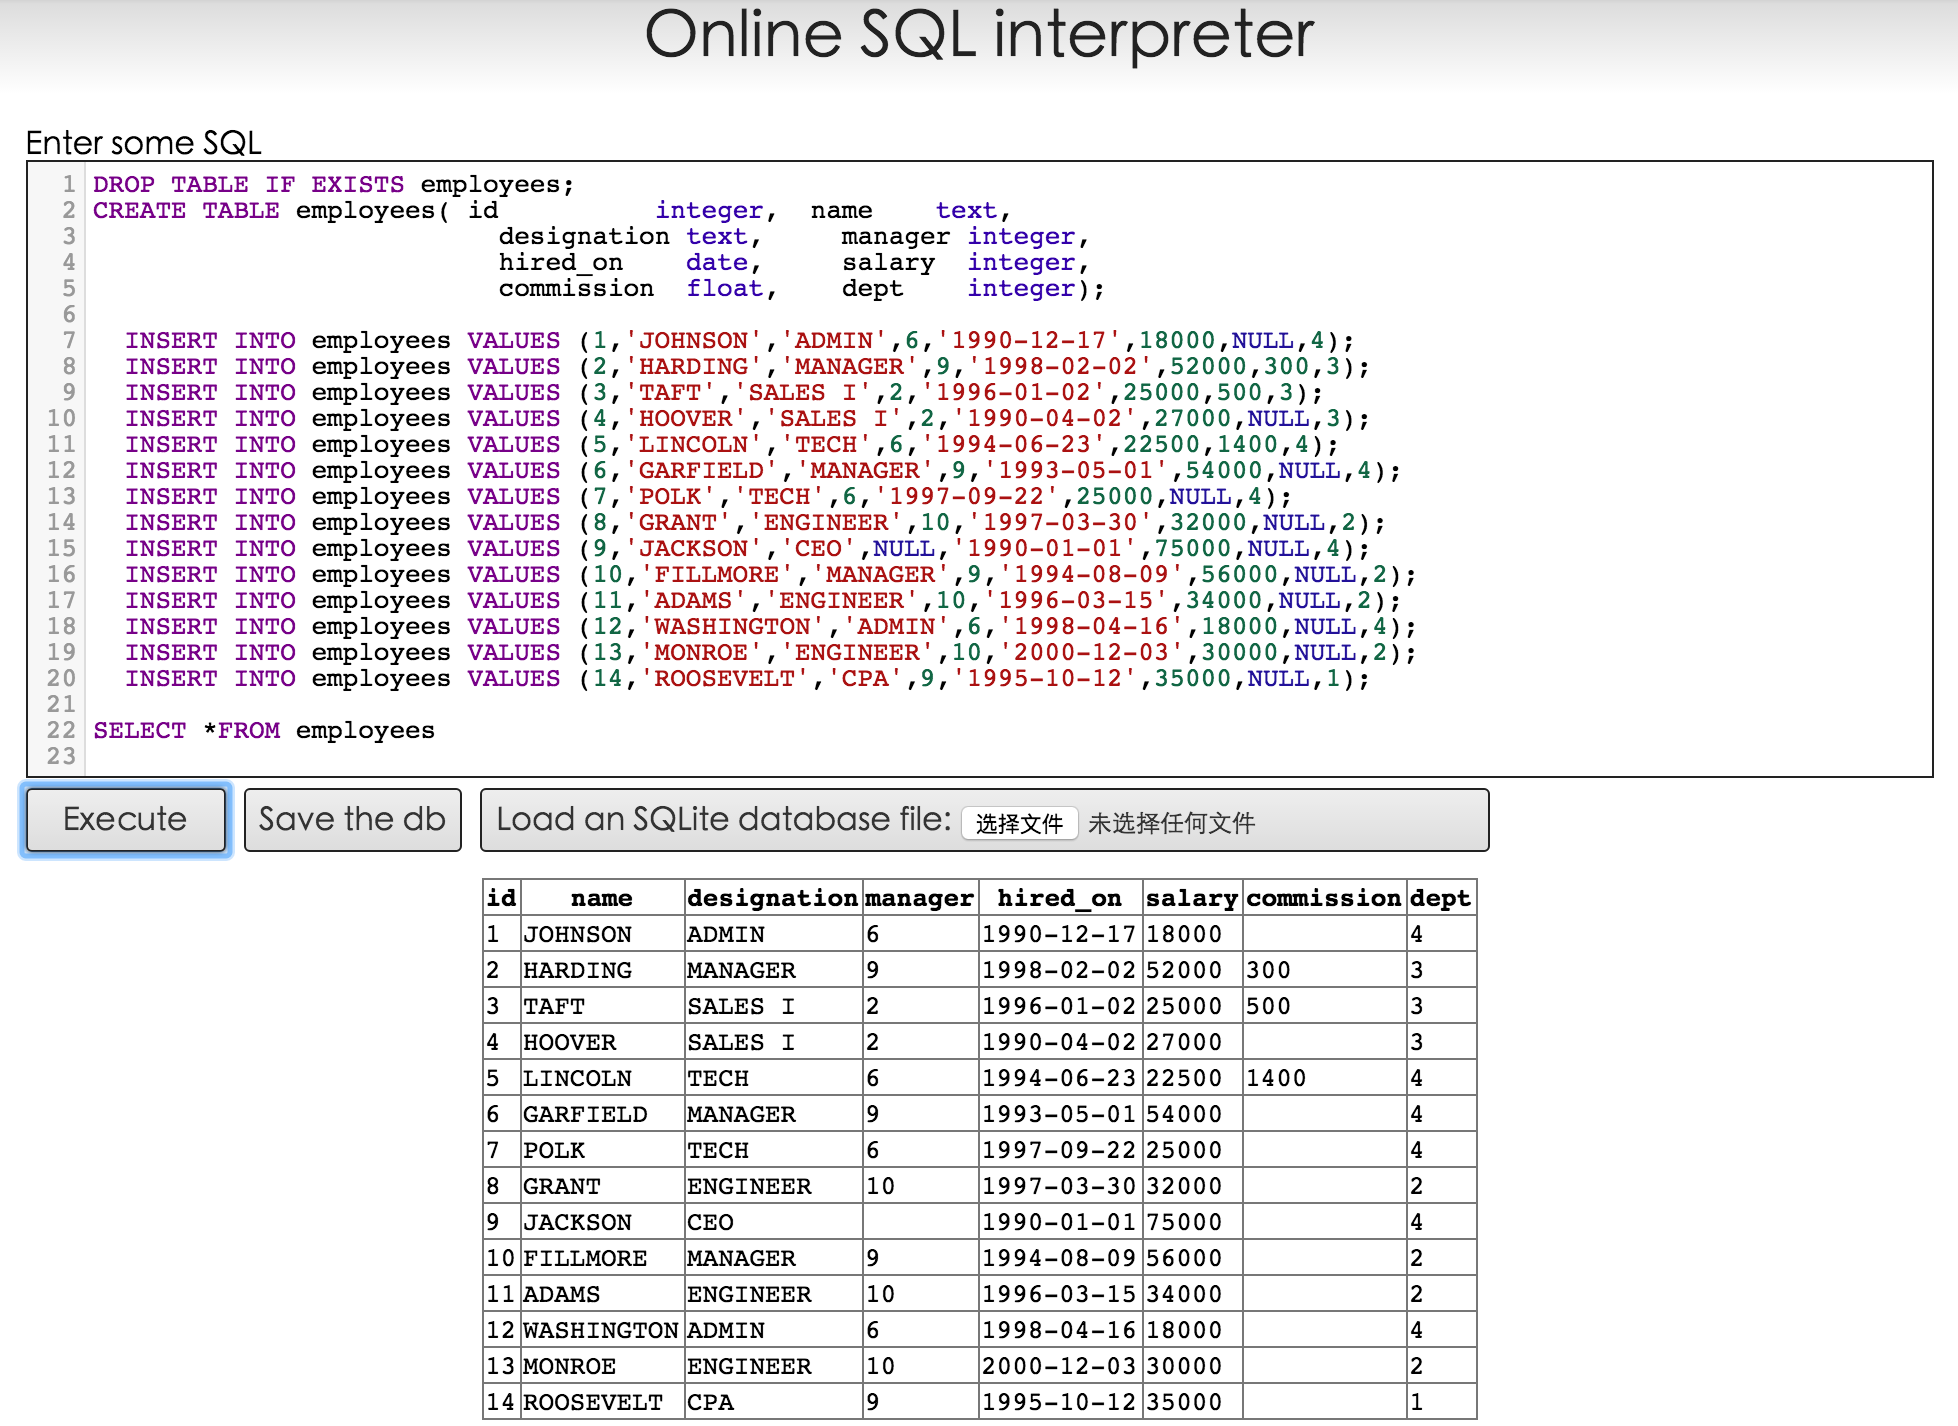
\includegraphics[width=450bp]{figure/pic/sqlite-sample-html.png}
    \caption{SQLite在浏览器中运行效果}
    \label{sqlite-html}
\end{figure}

该Web页面的上方是一个textarea,可以编写SQL代码,编写好自己的SQL代码之后,点击Execute按钮,可以让代码运行。下方的文本区是用来显示SQLite执行SQL代码的结果的,和命令行sqlite3的终端窗口作用相同。